\documentclass{article}

\usepackage{graphicx}
\usepackage{tikz}
\usepackage{tikzsymbols}
\usetikzlibrary{calc,patterns,shapes.geometric}
\pagestyle{empty}
\usepackage[margin=0pt]{geometry}
\geometry{papersize={14in,12in}}

\def\centerarc[#1](#2)(#3:#4:#5){\draw[#1] ($(#2)+({#5*cos(#3)},{#5*sin(#3)})$) arc (#3:#4:#5);}

\begin{document}
	\begin{figure}
		\centering
		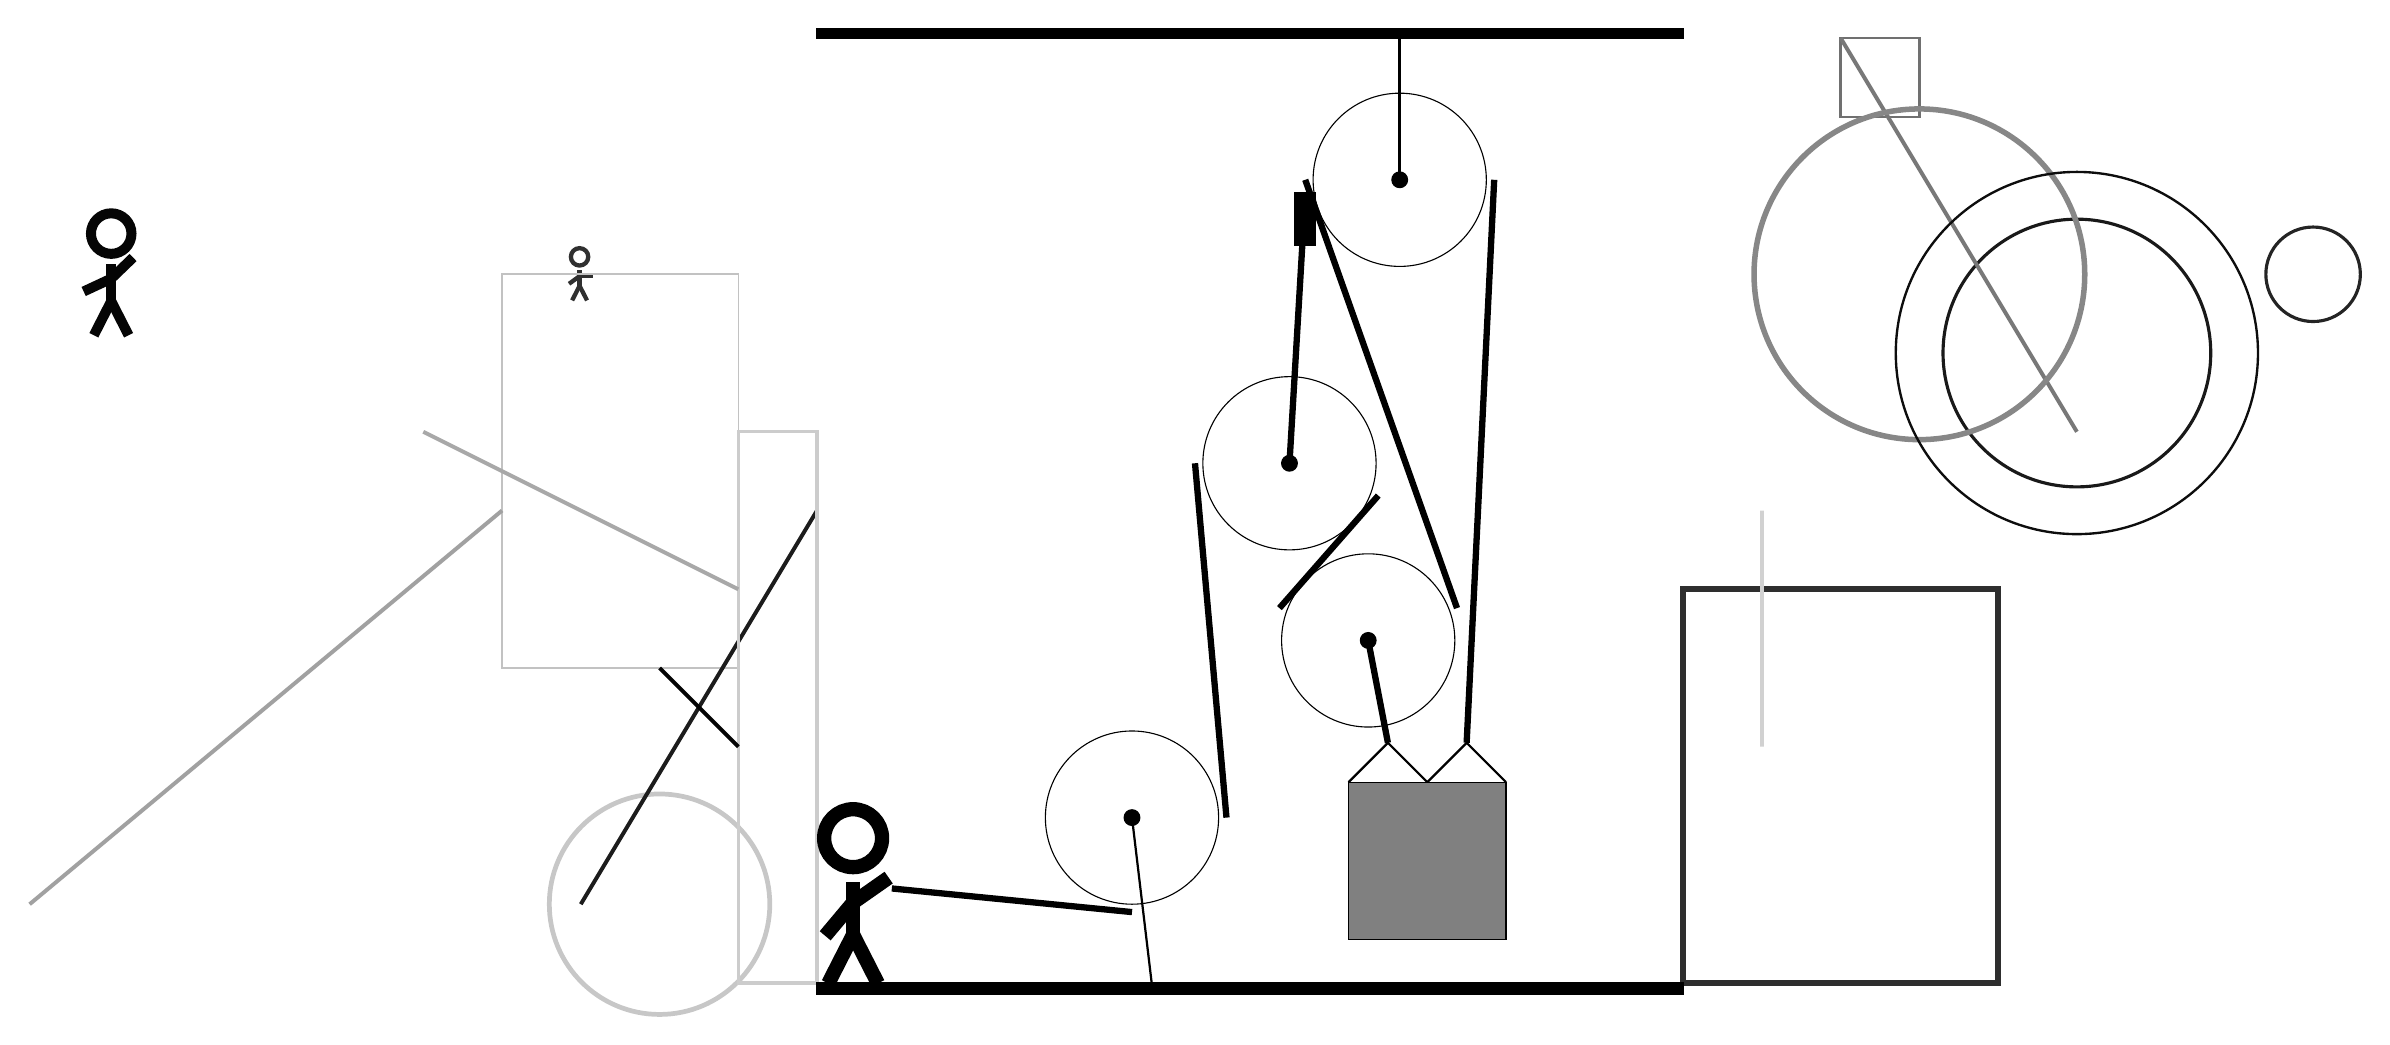
\begin{tikzpicture}
			%%%%% START %%%%%
			
			\draw[fill=black] (-6, 9) rectangle (5, 9.125);
			
			\draw (0, 3.6) circle (1.1);
			\draw[fill=black] (0, 3.6) circle (0.1);
			
			\draw (1, 1.35) circle (1.1);
			\draw[fill=black] (1, 1.35) circle (0.1);
			
			\draw (1.4, 7.2) circle (1.1);
			\draw[fill=black] (1.4, 7.2) circle (0.1);
			\draw[very thick] (1.4, 7.2) -- (1.4, 9);
			
			\draw (-2, -0.9) circle (1.1);
			\draw[fill=black] (-2, -0.9) circle (0.1);
			\draw[thick] (-2, -0.9) -- (-1.75, -3);
			
			
			\draw[thick]  (0.75, -0.45) -- (1.25, 0.05) -- (1.75, -0.45) -- (2.25, 0.05) -- (2.75, -0.45);
			\draw[fill=black!50] (0.75, -0.45) rectangle (2.75, -2.45);
			\draw[line width=0.8mm] (-5.05, -1.8) -- (-2, -2.1);
			\centerarc[line width=0.8mm](-2, -0.9)(270:360:1.2000000000000002);
			\draw[line width=0.8mm] (-0.8, -0.9) -- (-1.2, 3.6);
			\draw[line width=0.8mm] (0, 3.6) -- (0.2, 7.0);
			\draw[line width=0.8mm, fill=black](0.1, 6.4) rectangle (0.3, 7.0);
			\centerarc[line width=0.8mm](0, 3.6)(-20:180:1.2000000000000002);
			\draw[line width=0.8mm] (1.1276, 3.1896) -- (-0.1276, 1.7604);
			\centerarc[line width=0.8mm](1, 1.35)(160:380:1.2000000000000002);
			\draw[line width=0.8mm] (2.1276, 1.7604) -- (0.2, 7.2);
			\draw[line width=0.8mm](1, 1.35) -- (1.25, 0.05);
			\centerarc[line width=0.8mm](1.4, 7.2)(0:180:1.2000000000000002);
			\draw[line width=0.8mm] (2.6, 7.2) -- (2.25, 0.05);
			
			\node[line width=0.2mm, color=black!98] at (-15, 6) {\Strichmaxerl[7][25][44]};
			
			\node[line width=0.7mm, color=black!81] at (-9, 6) {\Strichmaxerl[3][36][0]};
			\draw[line width=0.3mm, color=black!56] (7, 9) rectangle (8, 8);
			\draw [line width=0.4mm, color=black!90](10, 5) circle (1.7);
			\draw[line width=0.7mm, color=black!82] (5, 2) rectangle (9, -3);
			
			\draw[line width=0.5mm, color=black!53](10, 4) -- (7, 9);
			\draw [line width=0.5mm, color=black!56](7, 3) circle (0.0);
			
			\draw[line width=0.5mm, color=black!18] (6, 0) rectangle (6, 3);
			\draw [line width=0.7mm, color=black!47](8, 6) circle (2.1);
			
			\draw[line width=0.2mm, color=black!24] (-7, 6) rectangle (-10, 1);
			\draw [line width=0.3mm, color=black!95](10, 5) circle (2.3);
			
			\draw [line width=0.6mm, color=black!22](-8, -2) circle (1.4);
			\draw [line width=0.4mm, color=black!86](13, 6) circle (0.6);
			\draw[line width=0.5mm, color=black!89](-9, -2) -- (-6, 3);
			\draw[line width=0.5mm, color=black!37](-10, 3) -- (-16, -2);
			\draw[line width=0.4mm, color=black!20] (-7, 4) rectangle (-6, -3);
			\draw[line width=0.5mm, color=black!34](-11, 4) -- (-7, 2);
			\draw[line width=0.5mm, color=black!99](-7, 0) -- (-8, 1);
			
			\node at (-5.5, -1.9) {\Strichmaxerl[10][50][35]};
			
			\draw[fill=black] (-6, -3) rectangle (5, -3.15);
			
			%%%%% END %%%%%
		\end{tikzpicture}
	\end{figure}	
\end{document}